\documentclass[letterpaper,11pt,oneside,reqno]{article}

%%%%%%%%%%%%%%%%%%%%%%%%%%%%%%%%%%%%%%%%%%%%%%%%%%%%%%%%%%%%

\usepackage[pdftex,backref=page,colorlinks=true,linkcolor=blue,citecolor=red]{hyperref}
\usepackage[alphabetic,nobysame]{amsrefs}

%%%%%%%%%%%%%%%%%%%%%%%%%%%%%%%%%%%%%%%%%%%%%%%%%%%%%%%%%%%%
%main packages
\usepackage{amsmath,amssymb,amsthm,amsfonts,mathtools}
\usepackage{graphicx,color}
\usepackage{upgreek}
\usepackage[mathscr]{euscript}

%equations
\allowdisplaybreaks
\numberwithin{equation}{section}

%tikz
\usepackage{tikz}
\usetikzlibrary{shapes,arrows,positioning,decorations.markings}

%conveniences
\usepackage{array}
\usepackage{adjustbox}
\usepackage{cleveref}
\usepackage{enumerate}
\usepackage{datetime}

%paper geometry
\usepackage[DIV=12]{typearea}

%%%%%%%%%%%%%%%%%%%%%%%%%%%%%%%%%%%%%%%%%%%%%%%%%%%%%%%%%%%%
%draft-specific
\synctex=1
% \usepackage{refcheck,comment}

%%%%%%%%%%%%%%%%%%%%%%%%%%%%%%%%%%%%%%%%%%%%%%%%%%%%%%%%%%%%
%this paper specific
\newcommand{\ssp}{\hspace{1pt}}

%%%%%%%%%%%%%%%%%%%%%%%%%%%%%%%%%%%%%%%%%%%%%%%%%%%%%%%%%%%%
\newtheorem{proposition}{Proposition}[section]
\newtheorem{lemma}[proposition]{Lemma}
\newtheorem{corollary}[proposition]{Corollary}
\newtheorem{theorem}[proposition]{Theorem}
%%%%%%%%%%%%%%%%%%%%%%%%%%%%%%%%%%%%%%%%%%%%%%%%%%%%%%%%%%%%
\theoremstyle{definition}
\newtheorem{definition}[proposition]{Definition}
\newtheorem{remark}[proposition]{Remark}
%%%%%%%%%%%%%%%%%%%%%%%%%%%%%%%%%%%%%%%%%%%%%%%%%%%%%%%%%%%%

\begin{document}
\title{Lectures on Random Matrices
(Spring 2025)
\\Lecture 13: Matching a Random Matrix Model to a Random Growth Model}


\date{Wednesday, April 9, 2025\footnote{\href{https://lpetrov.cc/rmt25/}{\texttt{Course webpage}}
$\bullet$ \href{https://lpetrov.cc/simulations/model/random-matrices/}{\texttt{Live simulations}}
$\bullet$ \href{https://lpetrov.cc/rmt25/rmt25-notes/rmt2025-l13.tex}{\texttt{TeX Source}}
$\bullet$
Updated at \currenttime, \today}}



\author{Leonid Petrov}


\maketitle

\section{Recap}

In the last lecture, we discussed various random growth models, and universal KPZ objects:
\begin{itemize}
	\item \textbf{Airy line ensemble} which arises as the scaling limit of the Dyson Brownian motion.
	\item \textbf{KPZ Equation} as a universal continuous random growth model.
	\item \textbf{Polynuclear growth model} (PNG) as a discrete analogue of the KPZ equation.
\end{itemize}

Then we briefly mentioned how the PNG model matches to a
last-passage percolation (LPP) model in
$\mathbb{R}^2_{\ge0}$ driven by the Poisson
point process as noise.
In this lecture, we are going to explore a different
LPP model which is defined on cells of $\mathbb{Z}_{\ge1}^{2}$, and
match it \emph{exactly} to the Wishart random matrix model which we have seen before in passing.
This matching is due to Dieker and Warren (2009)
\cite{dieker2008largest}, who proved it
in the context
of deformed random matrix spectra,
as suggested in
\cite{BorodinPeche2009}.
The key to this matching is a \emph{dynamical} perspective
on both the LPP and the random matrix models, which allows us to
match Markov chains in the two models, and not simply the distributions.

Throughout the discussion, we will consider the ``spiked'', multiparameter models,
which naturally include finite-rank deformations.

\section{The spiked Wishart ensemble}
\label{sec:Wishart}

\subsection{Definition of the spiked Wishart process}
\label{sub:Wishart_process}

Recall that a (complex) \emph{Wishart matrix} $M$ of dimension
$n$ with $t$ degrees of freedom (and identity covariance)
can be represented as $M = X X^*$, where $X$ is an $n\times
t$ random matrix with independent complex Gaussian entries.
Clearly, $M$ is a positive-semidefinite Hermitian matrix of
size $n\times n$. The eigenvalues
$(\lambda_1,\dots,\lambda_N)$ (with $\lambda_1\ge \cdots \ge
\lambda_N \ge 0$) have the joint density of the
\emph{Laguerre orthogonal polynomial ensemble} ($\beta=2$).
Now we introduce a more
general model where the covariance of the underlying
Gaussian matrix is not identity but has a
perturbation (a ``spike'').

\begin{definition}[Generalized Wishart ensemble with parameters $(\pi,\hat\pi)$]\label{def:Wishart}
Fix a positive integer $n$. Let $\pi=(\pi_1,\dots,\pi_n)$ be a fixed $n$-tuple of \emph{positive} real parameters, and let $\hat\pi = (\hat\pi_1,\hat\pi_2,\dots)$ be a sequence of \emph{nonnegative} real parameters (possibly infinite in length). We define an array of complex random variables $\{A_{ij}: 1\le i\le n, j\ge 1\}$ such that under the probability measure $P^{\pi,\hat\pi}$:
\begin{itemize}\item The $A_{ij}$ are independent for all $1\le i\le n$ and $j\ge 1$.
\item Each $A_{ij}$ is a complex Gaussian with mean $0$ and variance $\mathrm{Var}(A_{ij}) = \frac{1}{\pi_i + \hat\pi_j}$ (i.e. $\Re A_{ij}, \Im A_{ij} \sim N(0,\frac{1}{2(\pi_i+\hat\pi_j)})$ independent).
\end{itemize}
For each integer $t\ge 0$, let $A(t)$ denote the $n\times t$ sub-matrix consisting of the first $t$ columns of $A$. We then define an $n\times n$ random Hermitian matrix
\[ M(t) := A(t)\,A(t)^*, \qquad t\ge 0, \]
with the convention $M(0)$ is the zero matrix. We call $\{M(t): t\ge 0\}$ the \textbf{generalized Wishart random-matrix process} with parameters $(\pi,\hat\pi)$.
\end{definition}

In particular, $M(t)$ has the form
\[ M(t) = \sum_{m=1}^t A^{(m)} (A^{(m)})^*, \]
where $A^{(m)}$ denotes the $m$-th column of $A$ (an
$n$-dimensional complex random vector with independent
entries of variance $1/(\pi_i+\hat\pi_m)$). When all $\pi_i=1$ and all
$\hat\pi_j=0$, $M(t)$ reduces to the classical complex
Wishart($n,t$) with identity covariance.

\begin{remark}
	The introduction of parameters $\pi$ and $\hat\pi$ allows
	for \textbf{finite-rank deformations of the covariance}: one
	can think of the $\pi_i$'s as baseline values (say $\pi_i=1$
	for all but a few coordinates), and a finite number of them
	being different from 1 corresponds to a finite-rank
	perturbation of the identity covariance matrix $\Sigma$ (the
	directions in which $\pi_i\neq 1$ are "spiked"
	eigen-directions). Similarly, $\hat\pi_j$ can be viewed as
	adding a rank-one perturbation associated with each column;
	if only finitely many of the $\hat\pi_j$ are nonzero, that
	corresponds to having a finite number of distinguished
	samples (or boundary inhomogeneities in the equivalent
	percolation model, as we will see).
\end{remark}

We emphasize that $M(t)$
depends on $t$ in a way that $M(t)$ and $M(t-1)$ are not
independent but are coupled through shared columns. Indeed
$M(t) = M(t-1) + A^{(t)}(A^{(t)})^*$, which is a rank-1
update of $M(t-1)$.

\medskip
Let us denote by $\lambda_1(t)\ge \lambda_2(t)\ge \cdots \ge
\lambda_n(t)\ge 0$ the eigenvalues of $M(t)$ in
non-increasing order (padded with zeros if $t < n$, since
$\mathrm{rank}(M(t)) \le t$). We will use the notation
$\operatorname{sp}(M(t)) =
(\lambda_1(t),\dots,\lambda_n(t))$ for the \emph{spectrum}
of $M(t)$, viewed as a vector in the \emph{Weyl chamber}
$\mathbb{W}^n = \{x=(x_1,\dots,x_n)\in\mathbb{R}^n: x_1 \ge x_2 \ge
\cdots \ge x_n\}$. We are particularly interested in the
\emph{largest eigenvalue process}
$\{\lambda_1(t):t\ge0\}$, i.e. the sequence of the top
eigenvalue as the number of samples $t$ grows. Our goal is
to describe the law of this process and to identify it with
a combinatorial growth model.

Before stating the main result, we need a fundamental
property of the eigenvalue sequence
$\operatorname{sp}(M(t))$ as $t$ increases, namely that it
forms a \emph{Markov chain} in $\mathbb{W}^n$.
See Problem~\ref{prob:Markov}.

We need another statement:
\begin{lemma}[Interlacing; Problem~\ref{prob:interlacing}]
\label{lemma:interlacing}
For each $t\geq 1$, the eigenvalues of $M(t)$ and $M(t-1)$ satisfy the interlacing property:
\begin{equation}
	\label{eq:interlace}
	\lambda_1(t) \geq \lambda_1(t-1) \geq \lambda_2(t) \geq \lambda_2(t-1) \geq \cdots \geq \lambda_n(t-1) \geq \lambda_n(t) \geq 0.
\end{equation}
\end{lemma}
We denote the relation \eqref{eq:interlace} by
\begin{equation}
	\label{eq:interlace-notation}
	\lambda(t) \succ \lambda(t-1).
\end{equation}

In other words, the eigenvalue \emph{Markov processes}
$\lambda(t)$, $t=0,1,2,\ldots $
form an interlacing array, where at each step of the Markov process,
a new row of the array is ``revealed''.
The interlacing property is parallel to
the uniform conditioning (Gibbs) property in the $\beta=2$ corners. Moreover,
one can check (Problem~\ref{prob:Gibbs}) that
in the null case
$\pi_i=1$ and $\hat\pi_j=0$,
the Wishart eigenvalue process satisfies the
uniform Gibbs property as well.

\subsection{Markov chain and transition kernel for eigenvalues}
We say a random process $\{X(t):t\ge0\}$ taking values in
$\mathbb{W}^n$ is an \emph{inhomogeneous Markov chain} if
for each $m<t$, the conditional law of $X(t)$ given
$(X(t-1)=x_{t-1},\;X(t-2)=x_{t-2},\dots,X(m)=x_m)$ depends
only on $x_{t-1}$ (and possibly on $t$). In other words, the
process has the Markov property but the transition kernel
may depend on the time step $t$. In our case, since at each
step $t$ a new column $A^{(t)}$ with variance parameters
$\{\pi_i+\hat\pi_t:1\le i\le n\}$ is added, the transition
law from $M(t-1)$ to $M(t)$ will indeed depend on the index
$t$ through $\hat\pi_t$. We denote by
$Q^{\pi,\hat\pi}_{t-1,t}(x,dy)$ the transition kernel: for
$x\in \mathbb{W}^n$ given as the eigenvalue vector of
$M(t-1)$, $Q^{\pi,\hat\pi}_{t-1,t}(x,\cdot)$ is the
distribution of $\operatorname{sp}(M(t))$.

The null case $\pi_i=1$ and $\hat\pi_j=0$ of $Q^{\pi,\hat\pi}_{t-1,t}(x,dy)$
was computed in \cite{defosseux2010orbit}, see also
\cite{forrester2006jacobians}.

\begin{theorem}
\label{thm:MarkovChain}
Fix an integer \(n\ge1\).  Let \(\pi=(\pi_1,\dots,\pi_n)\) be a strictly positive \(n\)-vector, and let \(\widehat\pi=(\widehat\pi_1,\widehat\pi_2,\dots)\) be any sequence of nonnegative real parameters.  Under the probability measure \(P^{\pi,\widehat\pi}\), the eigenvalues of the \(n\times n\) generalized Wishart matrices \(\{M(t)\}_{t\ge0}\) form a time-inhomogeneous Markov chain \(\{\mathrm{sp}(M(t))\}_{t\ge0}\) in the Weyl chamber
\[
\mathbb{W}^n
\;=\;
\bigl\{\,x=(x_1,\dots,x_n)\in\mathbb{R}^n_{\ge0}:
x_1\ge x_2\ge\cdots\ge x_n\bigr\}.
\]
More precisely, writing \(x=\mathrm{sp}(M(t-1))\) and \(y=\mathrm{sp}(M(t))\), the one-step transition law from time \((t-1)\) to \(t\) is absolutely continuous on the interior of \(\mathbb{W}^n\) and can be factored as
\begin{equation}
\label{eq:transition-density}
Q_{t-1,t}^{\pi,\widehat\pi}(x,\,dy)
\;=\;
\Bigl[\,
\prod_{i=1}^n \bigl(\pi_i+\widehat\pi_{t}\bigr)
\Bigr]
\cdot
\frac{h_{\pi}(y)}{h_{\pi}(x)}
\;\exp\Bigl(-(\widehat\pi_{t}-1)\sum_{i=1}^n (y_i - x_i)\Bigr)
\;\times\;Q^{(0)}\bigl(x,\,dy\bigr),
\end{equation}
where
\begin{itemize}
\item \(\displaystyle Q^{(0)}\bigl(x,\,dy\bigr)\) is the \emph{standard} (null-spike) Wishart transition kernel, given explicitly by
	\begin{equation}
		\label{eq:Q0}
Q^{(0)}(x,\,dy)
\;=\;
\frac{\Delta(y)}{\Delta(x)}\;\exp\Bigl(\,-\sum_{i=1}^n (y_i - x_i)\Bigr)\,
\mathbf{1}_{\{x\prec y\}}\;dy,
\end{equation}
with \(\Delta(z)=\prod_{1\le i<j\le n}(z_i - z_j)\) the Vandermonde determinant.

\item The function \(h_{\pi}\) is the (continuous) Harish-Chandra orbit integral factor
\[
h_{\pi}(z)
\;=\;
\frac{(-1)^{\binom n2}}{0! 1! \cdots (n-1)! }
\frac{\det\bigl(e^{-\pi_i\,z_j}\bigr)_{i,j=1}^n}{\Delta(\pi)\,\Delta(z)}.
\]
Note that $h_\pi(0)=1$.
\end{itemize}
In particular, the chain starts from \(\mathrm{sp}(M(0))=0\) (the zero matrix).
\end{theorem}

\begin{proof}[Sketch of proof; see \cite{dieker2008largest}]
	First of all, random-matrix arguments
	\cite{defosseux2010orbit}, \cite{forrester2006jacobians} show that the
	theorem holds for the null case $\pi_i=1$ and $\hat\pi_j=0$.
	The Radon-Nikodym derivative of the transition kernel
	factors through the diagonal entries of the matrix,
	and can be written in terms of the eigenvalues via
	the HCIZ integral.
	This yields an explicit factor multiplying the null-case
	transition density.
\end{proof}



\begin{remark}[Problem~\ref{prob:CauchyBinet}]
\label{rem:CauchyBinet}
In order to see directly that the family $\bigl\{Q^{\pi,\hat{\pi}}_{t-1,t}\bigr\}$ of transition kernels does indeed define Markov transitions (that is, each $Q^{\pi,\hat{\pi}}_{t-1,t}(x,\cdot)$ is a probability measure for every $x$), one can use the fact that
\[
	\mathbf{1}_{z \prec z'}
\;=\;
\det\bigl[\mathbf{1}_{z_i < z'_j}\bigr],
\]
along with the Cauchy--Binet (or Andr\'eief) identity:
\[
\int_{\mathbb{W}^N}
\det[\xi_i(z_j)]\,
\det[\psi_j(z_i)]
\,dz
\;=\;
\det\Bigl[
\int_{\mathbb{R}}
\xi_i(z)\,\psi_j(z)\,dz
\Bigr].
\]
Applying this to
\eqref{eq:transition-density}--\eqref{eq:Q0}
yields a sequence of integrals
of the exponential densities
of the form $e^{-(\pi_i+\hat \pi_t)y}$.
This yields the normalizing factor
$\prod_{i,j}(\pi_i+\hat \pi_j)$,
and confirms
that each transition kernel
integrates to one, in line with the notation and
factorization in Theorem~\ref{thm:MarkovChain}.
\end{remark}

The fixed-time distribution of the eigenvalues
in the null case $\pi_i=1$ and $\hat\pi_j=0$ is
given by the Laguerre orthogonal polynomial ensemble. For example, for $t\ge n$, we have
\begin{equation}
	\label{eq:Laguerre}
	\operatorname{Prob}(\operatorname{sp}(M(t))\in dy)
	=
	\frac{1}{Z}\prod_{i<j}(y_i-y_j)^2
	\prod_{i=1}^n y_i^{t-n} e^{-y_i}.
\end{equation}
For the non-null case, see Problem~\ref{prob:Wishart_non_null}.

\section{The exponential LPP model}

We now turn to a seemingly different probabilistic model: a
model of random paths in a grid with random weights. Fix an
integer $n$. Consider an infinite array of independent,
nonnegative random weights $\{W_{ij}: i\ge 1,\ 1\le j\le n\}$ defined under the probability measure $P^{\pi,\hat\pi}$,
where each $W_{ij}$ is an independent random variable with
an \emph{exponential} distribution of rate $(\pi_i +
\hat\pi_j)$.
Note that $\mathbb{E}[W_{ij}] = \frac{1}{\pi_j+\hat\pi_i}$.
These rates $(\pi_j+\hat\pi_i)$ are chosen deliberately to
mirror the variance parameters of $A_{ij}$ in the
generalized Wishart model (Definition \ref{def:Wishart}).

We interpret $\{W_{ij}\}$ as random weights on the vertices of a directed lattice in the first quadrant. Specifically, consider the set of lattice points
\[ \{(i,j): i=1,\ldots,t,\ldots ,\ j=1,\dots,n\}.\]
We say a path $\Gamma$ is an \emph{up-right path} from
$(1,1)$ to $(t,n)$ if it is a sequence of lattice points
starting at $(1,1)$ and ending at $(t,n)$, with steps either
one step to the right or one step up. Since each step
either increases the column index by 1 or the row index by
1, any such path from $(1,1)$ to $(t,n)$ must consist of
$(t-1)$ right-steps and $(n-1)$ up-steps, for a total of
$(t+n-2)$ steps. We define the \emph{weight} of a path
$\Gamma$ to be the sum of the $W_{ij}$ along its vertices:
\[ \mathcal{W}(\Gamma) := \sum_{(i,j)\in \Gamma} W_{ij}, \]
where by $(i,j)\in \Gamma$ we mean that the vertex $(i,j)$ is visited by the path $\Gamma$. The random variable of interest is the \emph{maximum total weight achievable among all such paths}, i.e.
\begin{equation}\label{eq:last-passage-time}
L(t,n) := \max_{\Gamma:\, (1,1)\to(t,n)} \; \mathcal{W}(\Gamma)\,.
\end{equation}
We call $L(t,n)$ the \emph{last-passage time} to $(t,n)$, in analogy with the usual terminology of growth models (if we interpret $W_{ij}$ as random passage times on a lattice, then the longest time to reach a certain site is given by the maximal weight path).

\begin{figure}[ht]
\centering
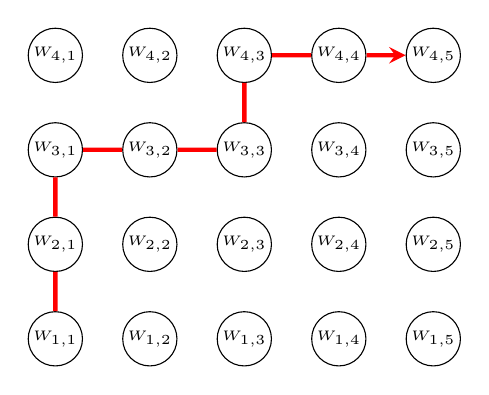
\begin{tikzpicture}[scale=1.2,>=stealth]
				% Draw a 4 (rows) by 5 (columns) grid of nodes.
				% We'll place row i = 1 at the bottom and i = 4 at the top,
				% and columns j=1..5 from left to right.
				% Each node is labeled with W_{i,j}.
				\foreach \i in {1,2,3,4} {
								\foreach \j in {1,2,3,4,5} {
												% Position nodes so that i=1 is bottom row, i=4 top row.
												\node[circle,draw,fill=white,inner sep=1pt]
																		(n\i-\j)
																		at (\j,\i)
																		{\tiny $W_{\i,\j}$};
								}
				}

				% Draw one example of an up-right path from (1,1) to (4,5).
				% It has exactly 3 "up" steps (increasing i) and 4 "right" steps (increasing j).
				\draw[ultra thick, red,->]
								(n1-1) -- (n2-1) -- (n3-1) -- % three steps up
								(n3-2) -- (n3-3) --           % two steps right
								(n4-3) --                     % one step up
								(n4-4) -- (n4-5);             % two steps right

				% Optionally, you can add arrows for all edges (to the right and upward)
				% if you want to depict the entire directed lattice structure.
				% E.g.:
				% \foreach \i in {1,...,4}{
				%   \foreach \j in {1,...,4}{
				%       \draw[->,black!30] (n\i-\j) -- (n\i-\the\numexpr\j+1\relax);
				%   }
				% }
				% \foreach \i in {1,...,3}{
				%   \foreach \j in {1,...,5}{
				%       \draw[->,black!30] (n\i-\j) -- (n\the\numexpr\i+1\relax-\j);
				%   }
				% }
\end{tikzpicture}
\caption{A portion of the lattice with vertex-weights $W_{i,j}$ and one up-right path.}
\label{fig:LPP_array}
\end{figure}


Indeed, it is immediate from the definition that the random
variables $L(t,n)$ satisfy the following random recursion:
\begin{equation}\label{eq:LPP-recursion}
L(i,j) = W_{ij} + \max\{\, L(i,j-1),\; L(i-1,j)\,\}\,,
\end{equation}
for $i>1, j>1$, with boundary conditions $L(t,1) =
\sum_{k=1}^t W_{k,1}$ and $L(1,i) =
\sum_{\ell=1}^i W_{1,\ell}$.
The recursion \eqref{eq:LPP-recursion} expresses
that the optimal path to $(i,j)$ either comes from below
(then last step is down, contributing $W_{ij}$ plus the
optimal weight to $(i,j-1)$) or from the left (last step is
right from $(i-1,j)$). It is the fundamental equation of
growth models, which is a part of the
\emph{Robinson--Schensted--Knuth insertion algorithm} in
combinatorics.


\begin{remark}
	The quantity $L(t,n)$ appears in many contexts besides the LPP.
	Namely,
it is also the total
service time in a series of $n$ exponential queueing servers
with $t$ customers (the \emph{Jackson network}
interpretation \cite{Baryshnikov_GUE2001}), and it is a
prototype of models in the KPZ universality class (often
called the \emph{exponential corner growth model}).
For the random growth interpretation \cite{johansson2000shape},
define the growing percolation cluster as
\begin{equation*}
\begin{split}
F_\tau\coloneqq
\left\{ (i,j)\colon L(j,i)\le t \right\} \subseteq \mathbb{Z}_{\ge1}^2,
\qquad \tau \in \mathbb{R}_{\ge0}.
\end{split}
\end{equation*}
Then this cluster grows by adding $1\times 1$ boxes
after exponential random times, when
each rate $\pi_j+\hat \pi_i$
exponential clock starts ticking
when the cluster reaches the two adjacent vertices
to $(i,j)$.
\end{remark}

Let us define the whole \emph{vector of last-passage times to the bottom row} at column $t$ as
\[ Z(t) := \big( L(t,1),\, L(t,2),\, \dots,\, L(t,n)\big)\,\in \mathbb{W}^n, \]
where we list the values in increasing order $L(t,1)\le
L(t,2)\le \cdots \le L(t,n)$.\footnote{We have $L(t,1)\le
\cdots\le L(t,n)$ almost surely because giving the path more
freedom to move down can only increase the maximum weight.
This is easily checked from \eqref{eq:LPP-recursion}. Thus
$Z(t)\in \mathbb{W}^n$ indeed.} In particular, $L(t,n)$ is
the largest component of $Z(t)$. The sequence
$\{Z(t):t\ge0\}$, with $Z(0)=(0,\dots,0)$, is a random
process in $\mathbb{W}^n$.

\begin{remark}
	The process $Z(t)$ is \textbf{not} the same as the
	Markov process of the spectra of the Wishart matrices
	$M(t)$. Instead, we should look at the maximal eigenvalues
	$\operatorname{sp}(M(t))_{\max}$
	of the $n\times n$ matrices $M(t)$, $t=0,1,\ldots$,
	and match them to the last-passage times
	$L(t,n)$, $t=0,1,\ldots$.
\end{remark}

In the next section, we will consider a discrete version of the
LPP model, and consider a crucial bijection --- the celebrated
\emph{Robinson--Schensted--Knuth (RSK) correspondence}.
In the next \href{https://lpetrov.cc/rmt25/rmt25-notes/rmt2025-l14.pdf}{Lecture 14}, we will
use this to complete the proof of the matching between the
Wishart process and the LPP with exponential weights.
That is, we are after the following result:
\begin{theorem}[\cite{dieker2008largest}]
	\label{thm:matching}
	The joint distribution of the last-passage times
	\begin{equation*}
		L(1,n),\;L(2,n),\ldots,L(t,n)
	\end{equation*}
	is the same as the joint distribution of the largest
	eigenvalues
	of the $n\times n$ Wishart matrices
	\begin{equation*}
		\operatorname{sp}(M(1))_{\max},\;\operatorname{sp}(M(2))_{\max},\ldots,\operatorname{sp}(M(t))_{\max}.
	\end{equation*}
\end{theorem}


\section{Geometric LPP and Robinson-Schensted-Knuth correspondence}

\subsection{Geometric LPP}

Throughout this section, we are interested in the
last-passage percolation with discrete weights $W_{ij}\in \mathbb{Z}_{\ge0}$,
which have the geometric distribution
\begin{equation}
	\label{eq:geometric}
	\operatorname{Prob}(W_{ij}=k) = \frac{(a_i b_j)^{k}}{(1 - a_ib_j)^{k+1}}, \qquad k=0,1,\ldots
\end{equation}
The last-passage times are defined by \eqref{eq:LPP-recursion},
the same as in the exponential case.

\subsection{Bijective mapping of arrays via toggles}
\label{sub:toggle}

We are now going to present the Robinson-Schensted-Knuth
correspondence via the operation called \emph{toggle}.
This exposition is different from the usual discussions in e.g.,
\cite{sagan2001symmetric}, \cite{fulton1997young},
and follows these \href{https://www.samuelfhopkins.com/docs/rsk.pdf}{notes by Sam Hopkins}.
Fix $t,n$, and consider the array $W=\{W_{ij}\}_{1\le i\le n, 1\le j\le t}$ of
nonnegative integers. We can think of $W$ as a realization of the geometric
environment, but for now let us assume that $W$ is a fixed array. See
\Cref{fig:LPP_array} for the order of indices.

We are going to inductively construct a bijection $\operatorname{RSK}$ between the array $W$ and another
array $R=\{R_{ij}\}_{1\le i\le n, 1\le j\le t}$ of nonnegative integers, which is
\emph{ordered}:
\begin{equation*}
	R_{i,j} \le R_{i,j+1}, \qquad R_{i,j} \le R_{i+1,j},\qquad \text{for all } i,j.
\end{equation*}
Note that this ordering means that the diagonals in $R$ interlace.

To define $\operatorname{RSK}$, we first define an elementary
operation called \emph{toggle} and denoted by $\operatorname{T}$.

\begin{definition}[Toggle]
	The toggle operation is a map $\operatorname{T}$ which takes in
	a nonnegative integer $w$ and
	a triple $(\lambda,\kappa,\mu)$ of sequences of nonnegative integers
	satisfying interlacing
	\begin{equation*}
		\lambda\succ \kappa\prec \mu.
	\end{equation*}
	The lengths of the sequences are differ by $0$ or $1$, and if necessary, we pad the
	sequences with $0$'s to make the interlacing make sense.
	The output of $\operatorname{T}$ is a triple $(\lambda,\nu,\mu)$, where
	$\lambda$ and $\mu$ are not changed, and $\nu$ is obtained from $\lambda,\mu,\kappa$,
	and $w$ as follows:
	\begin{equation*}
		\nu_1=w+\max(\lambda_1,\mu_1),\qquad
		\nu_i=\max(\lambda_{i},\mu_i)+\min(\lambda_{i-1},\mu_{i-1})-\kappa_{i-1},\qquad
		\text{for } i\ge 2.
	\end{equation*}
\end{definition}
Define $|\kappa|\coloneqq \kappa_1+\kappa_2+\cdots$, and similarly for
$\lambda,\mu,\nu$.

\begin{proposition}
	\label{prop:toggle_weight_preservation}
	If $(\lambda,\nu,\mu)=\operatorname{T}(w;\lambda,\kappa,\mu)$, then
	$\lambda\prec\nu\succ \mu$, and
	\begin{equation*}
		|\nu|=w+|\lambda|+|\mu|-|\kappa|.
	\end{equation*}
\end{proposition}
\begin{proof}
	See Problem~\ref{prob:toggle_weight_preservation}.
\end{proof}


Now, define $R=\operatorname{RSK}(W)$ as follows.
We will build $R$
by sequentially modifying the array $W$,
starting from the bottom-left corner $(1,1)$ and moving
by adding one box at a time.
We represent the partially filled $R$ array as a collection of interlacing sequences.
Let $R^{(i,j)}$ denote the already constructed part of $R$, where we are adding a
box $(i,j)$. Then, we modify the diagonal containing
$(i,j)$ by applying the toggle operation to the weight $w=W_{i,j}$ and the three diagonals
\begin{equation*}
	\lambda^{(i,j)} = \{R^{(i,j)}_{i-k+1,j-k}\}_{k\ge1}, \quad
	\mu^{(i,j)} = \{R^{(i,j)}_{i-k,j-k+1}\}_{k\ge1}, \quad
	\kappa^{(i,j)} = \{R^{(i,j)}_{i-k,j-k}\}_{k\ge1}.
\end{equation*}
\begin{figure}[ht]
\centering
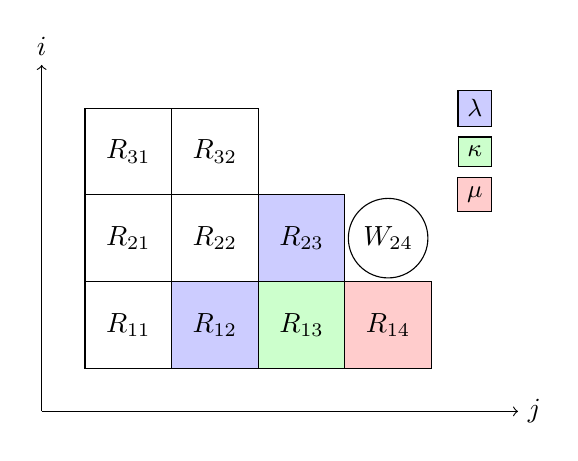
\begin{tikzpicture}[scale=1.1]
% Draw coordinate axes
\draw[->] (0,0) -- (5.5,0) node[right] {$j$};
\draw[->] (0,0) -- (0,4) node[above] {$i$};

% Bottom row (i=1)
\foreach \j in {1,2,3,4} {
	\node[rectangle,draw,minimum size=1.1cm] (R1\j) at (\j,1) {$R_{1\j}$};
}
% Middle row (i=2) - including the box being added
\foreach \j in {1,2,3} {
					\node[rectangle,draw,minimum size=1.1cm] (R2\j) at (\j,2) {$R_{2\j}$};
				}
				% Top row (i=1)
				\foreach \j in {1,2} {
					\node[rectangle,draw,minimum size=1.1cm] (R3\j) at (\j,3) {$R_{3\j}$};
					}

					\node[circle,draw] at (4,2) {$W_{24}$};

																	% Highlight lambda cells
																	\node[rectangle,draw,fill=blue!20,minimum size=1.1cm] at (3,2) {$R_{23}$};
																	\node[rectangle,draw,fill=blue!20,minimum size=1.1cm] at (2,1) {$R_{12}$};

																	% Highlight kappa cells
																	\node[rectangle,draw,fill=green!20,minimum size=1.1cm] at (3,1) {$R_{13}$};

																	% Highlight mu cells
																	\node[rectangle,draw,fill=red!20,minimum size=1.1cm] at (4,1) {$R_{14}$};

																	% Add a legend
																	\node[draw,fill=blue!20] at (5,3.5) {\small $\lambda$};
																	\node[draw,fill=green!20] at (5,3) {\small $\kappa$};
																	\node[draw,fill=red!20] at (5,2.5) {\small $\mu$};

				\end{tikzpicture}
				\caption{Illustration of the RSK toggle operation,
					with $w=W_{24}$ being added to the array $R$,
					and $\lambda=(R_{23},R_{12})$,
					$\kappa=(R_{13})$, $\mu=(R_{14})$.}
					\label{fig:toggle}
\end{figure}

The next statement is straightforward:
\begin{proposition}
	The toggle operation $\operatorname{T}$ is a bijection
	\begin{equation*}
		\mathbb{Z}_{\ge0}\times
		\left\{ (\lambda,\kappa,\mu)\colon \lambda\succ \kappa\prec \mu \right\}
		\leftrightarrow
		\left\{ (\nu,\lambda,\mu)\colon \lambda\prec\nu \succ \mu \right\}.
	\end{equation*}
	Consequently, the map $\operatorname{RSK}$ is a bijection
	between nonnegative
	arrays $W$ and ordered nonnegative arrays $R$.
\end{proposition}

\begin{proposition}
\label{prop:RSK_independence_of_order}
	The bijection $\operatorname{RSK}$ does not depend on the order
	of adding the boxes to the array $R$.
\end{proposition}
\begin{proof}
	See Problem~\ref{prob:RSK_independence_of_order}.
\end{proof}

\subsection{Weight preservation}

Define
the row and column sums in $W$ by 
\begin{equation*}
	\mathrm{row}_i\coloneqq \sum_{j=1}^t W_{ij}, \qquad
	\mathrm{col}_j \coloneqq \sum_{i=1}^n W_{ij}.
\end{equation*}
Also define the diagonal sums in $R$ by
\begin{equation*}
	\mathrm{diag}_{i,j}\coloneqq \sum_{k=0}^{\min(i,j)-1}R_{i-k,j-k}.
\end{equation*}

\begin{proposition}[RSK weight preservation]
	Under the bijection $\operatorname{RSK}$, we have
\end{proposition}
\begin{proof}
	
\end{proof}

In the next
\href{https://lpetrov.cc/rmt25/rmt25-notes/rmt2025-l14.pdf}{Lecture
14}, we will consider the effect of applying the RSK 
to the array $W$ of independent geometric random variables.


\appendix
\setcounter{section}{12}

\section{Problems (due 2025-04-29)}

\subsection{Wishart Markov chain}
\label{prob:Markov}

In the null case $\pi_i = 1$ and $\hat\pi_j = 0$,
show that the
process $\operatorname{sp}(M(t))$
defined in \Cref{sub:Wishart_process}
is a Markov chain.

\medskip
\noindent
\textbf{Hint:} Use diagonalization and
the fact that the Wishart matrix distribution is invariant under
conjugations by unitary matrices,
similarly to how we did it for the Dyson Brownian motion in
\href{https://lpetrov.cc/rmt25/rmt25-notes/rmt2025-l10.pdf}{Lecture 10}.


\subsection{Interlacing}
\label{prob:interlacing}

Prove \Cref{lemma:interlacing}.

\medskip
\noindent
\textbf{Hint:} You can use the minimax definition of the eigenvalues to show the interlacing.

\subsection{Gibbs property}
\label{prob:Gibbs}

Show that in the null case \(\pi_i = \hat\pi_j = 0\), the
Wishart eigenvalue process
from \Cref{sub:Wishart_process}
has the Gibbs conditioning property:
when conditioned on the values of
$\lambda(t)$, the joint distribution of
all the eigenvalues
$\left\{ \lambda(s)\colon s=0,1,\ldots,t-1  \right\}$
is uniform in the Gelfand--Tsetlin polytope
determined by $\lambda(t)$ and the interlacing.


\subsection{Transition kernels integrate to one}
\label{prob:CauchyBinet}

Complete the argument outlined in \Cref{rem:CauchyBinet}
that the transition densities $Q^{\pi,\hat\pi}_{t-1,t}(x,dy)$
integrate to one in $y$.


\subsection{Distribution of the eigenvalues}
\label{prob:Wishart_non_null}

Find the density
$\operatorname{Prob}\left( \operatorname{sp}(M(t))\in dy \right)/dy$
of the spiked Wishart ensemble
at an arbitrary fixed time $t$.
For this, you can multiply the transition operators
$Q^{\pi,\hat\pi}_{t-1,t}$ from \Cref{thm:MarkovChain}.


\subsection{Weight preservation under toggle}
\label{prob:toggle_weight_preservation}

Prove \Cref{prop:toggle_weight_preservation}.


\subsection{RSK independence of order}
\label{prob:RSK_independence_of_order}

Prove Proposition \ref{prop:RSK_independence_of_order}, which states that the bijection $\operatorname{RSK}$ does not depend on the order of adding the boxes to the array $R$.

\medskip
\noindent
\textbf{Hint:} Toggle operations commute when they act on non-overlapping diagonals.



% \subsection{Generalized RSK and LPP}
% Consider the inhomogeneous geometric LPP model with site rates \(\{a_i b_j\}\).  Show directly (without passing to the continuous limit) that the vector of last-passage times \(\{Y(i,n)\}\) forms a Markov chain in the Gelfand--Tsetlin cone, and write down its transition probability in factorized form.

\subsection{Asymptotics: BBP phase transition}
Review the proof of the BBP transition for a rank-1 spiked
Wishart matrix (or the rank-1 inhomogeneous corner-growth
model).  Show how to compute the large-\(n\) limiting
distribution of the top eigenvalue in the critical case
Identify the
limit law as a \emph{deformed Airy kernel} (or equivalently
a shifted Airy$_2$ process).




\bibliographystyle{alpha}
\bibliography{bib}


\medskip

\textsc{L. Petrov, University of Virginia, Department of Mathematics, 141 Cabell Drive, Kerchof Hall, P.O. Box 400137, Charlottesville, VA 22904, USA}

E-mail: \texttt{lenia.petrov@gmail.com}

\end{document}
